\documentclass{beamer}

\usetheme{CambridgeUS}

\usepackage{listings}
\usepackage{amssymb}
%\usepackage[cmex10]{amsmath}

\usepackage[export]{adjustbox}
\usepackage{bm}
\def\inputGnumericTable{} 

\usepackage[latin1]{inputenc}                                 
\usepackage{color}                                            
\usepackage{array}   
\usepackage{longtable}
\usepackage{enumitem}
\usepackage{calc}                                             
\usepackage{multirow}                                         
\usepackage{hhline}                                           
\usepackage{ifthen}  
\usepackage{mathtools}
\usepackage{tikz}
\usepackage{listings}
\usepackage{color}                                            %%
\usepackage{array}                                            %%
\usepackage{caption} 
\usepackage{graphicx}
\graphicspath{{images/}}
\captionsetup[table]{skip=3pt} 

 

\title{A1110 Assignment 8 }
\author{Tejal Kulkarni \\ CS21BTECH11058 \\\vspace*{20pt} CBSE Probability Grade 12 }

\begin{document}

%\newcommand{\solution}{\noindent \textbf{Solution: }}
\providecommand{\pr}[1]{\ensuremath{\Pr\left(#1\right)}}
\providecommand{\cdf}[2]{\ensuremath{\text{F}_{#1}\left(#2\right)}}
\providecommand{\qfunc}[1]{\ensuremath{Q\left(#1\right)}}
\providecommand{\sbrak}[1]{\ensuremath{{}\left[#1\right]}}
\providecommand{\lsbrak}[1]{\ensuremath{{}\left[#1\right.}}
\providecommand{\rsbrak}[1]{\ensuremath{{}\left.#1\right]}}
\providecommand{\brak}[1]{\ensuremath{\left(#1\right)}}
\providecommand{\lbrak}[1]{\ensuremath{\left(#1\right.}}
\providecommand{\rbrak}[1]{\ensuremath{\left.#1\right)}}
\providecommand{\cbrak}[1]{\ensuremath{\left\{#1\right\}}}
\providecommand{\lcbrak}[1]{\ensuremath{\left\{#1\right.}}
\providecommand{\rcbrak}[1]{\ensuremath{\left.#1\right\}}}
\newcommand*{\permcomb}[4][0mu]{{{}^{#3}\mkern#1#2_{#4}}}
\newcommand*{\perm}[1][-3mu]{\permcomb[#1]{P}}
\newcommand*{\comb}[1][-1mu]{\permcomb[#1]{C}}
\renewcommand{\thetable}{\arabic{table}} 

\begin{frame}
    \titlepage
\end{frame}

\begin{frame}{Outline}
  \tableofcontents
\end{frame}

\section{Question}
\begin{frame}{Question}
 \textbf{Example 32:}Ten eggs are drawn successively with replacement from a lot containing 10\% defective eggs. Find the probability that there is atleast one defective egg.    
\end{frame}

\section{Solution}
\begin{frame}{Defining random variables}
Let $X_{i}, 1 \leq i \leq N$ be N Bernoulli random variables.  Then,
\begin{align}   
\pr{X_i = k} = 
\begin{cases}
1 - p, & k = 0 \\
p, & k = 1 \\
0, & \textrm{otherwise}
\end{cases}
\label{1}
\end{align}
Let Y be a random variable such that,
\begin{equation}
    Y = \sum_{i = 1}^{i = N}X_i 
\end{equation}
\end{frame}
\begin{frame}{Moment generating Function of X}
    Using equation \eqref{1}, the moment generating function of $X_{i}$ can be given as,
\begin{align}
    M_Z(X_i) &= \sum_{k = -\infty}^{k = \infty}z^{-k}P_X(k) \\
             &= P_X(0) + z^{-1}P_X(1) \\
             &= (1 - p) + pz^{-1}
\end{align}
\end{frame}
\begin{frame}{Moment generating Function of $X_i$}
   Since all the $X_i$ are independent and identically distributed, the moment generating function of $Y$ is
\begin{align}
M_Y(Z) &= E(Z^{-Y}) = E(Z^{-\sum_{i = 1}^{i = N}X_i}) \\
       &= \prod_{i = 1}^{i = N}E(Z^{-X_i}) \\
       &= \sbrak{(1 - p) + pz^{-1}}^N \\
       &= \sum_{k = 0}^{k = N}z^{-k}(\binom{N}{k}(1 - p)^{N - k}p^k)
\end{align} 
\end{frame}

\begin{frame}{PMF and CDF of Y}
    The PMF of the Binomial random variable $Y$ is
\begin{align}
\pr{Y = k} = 
\begin{cases}
\binom{N}{k}(1 - p)^{N - k}p^k, & 0 \leq k \leq N \\
0, & \textrm{otherwise}
\end{cases}
\label{pmf-Y}
\end{align}
Therefore, the CDF of $Y$ is given by,
\begin{align}
&\cdf{Y}{k} = \sum_{i = -\infty}^{i = k}\pr{Y = i} \nonumber\\
&=\begin{cases}
0, & k < 0 \\
\sum_{K = 0}^{K = k}\binom{N}{K}(1 - p)^{N - K}p^K, & 0 \leq k < N \\
1, & k \geq N
\end{cases}
\label{cdf-Y}
\end{align}
\end{frame}

\begin{frame}{Given Information}
   Now,let Y be the binomial random variable denoting the number of defective eggs drawn.Hence $N = 10$ and,
\begin{equation}
    \text{Probability of success} = p = \frac{10}{100} = \frac{1}{10} 
\end{equation}
To find:
\begin{equation}
    \pr{\text{atleast one defective egg}} = \pr{Y \ge 1} 
\end{equation}
\end{frame}
\begin{frame}{Calculation of answer}
Now,
\begin{equation}
    \pr{Y \ge 1} = \sum_{k=0}^{10} \pr{Y = k} - \pr{Y = 0}
\end{equation}
Also,
\begin{align}
    \sum_{k=0}^{10} \pr{Y = k} &= 1 \\
    \implies \pr{Y \ge 1} &= 1 - \pr{X = 0}
\end{align}
Using \eqref{pmf-Y},
\begin{align}
 \pr{Y \ge 1} &= 1 - \comb{10}{0}\brak{\frac{1}{10}}^0\brak{\frac{9}{10}}^{10}\\
            &= 1 - \frac{9^{10}}{10^{10}} = \boxed{0.651}
\end{align} 
\end{frame}

\begin{frame}{Graphs - PMF and CDF of Y}
    \begin{figure}[!ht]
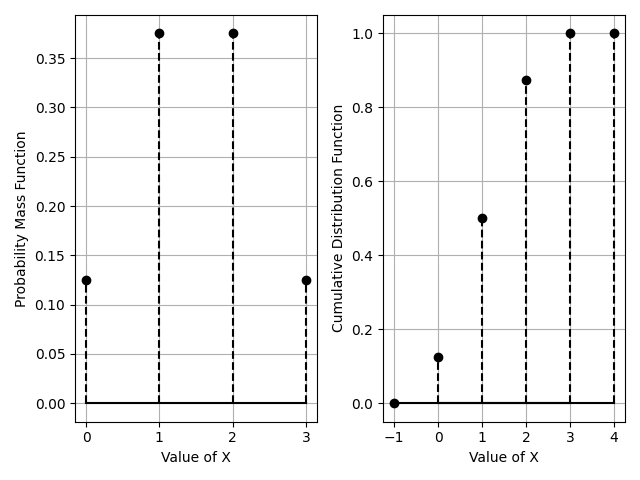
\includegraphics[height=0.7\textheight, width=0.7\textwidth, keepaspectratio]{PMF&CDF.png}
\caption{PMF and CDF for the given situation.}
\label{Fig 1}
\end{figure}
\end{frame}


\end{document}